\chapter{芳香环、药物与染料}

\begin{kaichang}
从你家的药箱里找一颗白色药片——比如最常见的退烧药对乙酰氨基酚。再去衣柜里翻一条蓝牛仔裤，或者一件颜色鲜艳的 T 恤。

一颗药、一块布，一个是吃的，一个是穿的，看上去八竿子打不着。可如果把它们各自最关键的分子放大几亿倍，你会看到同一个零件：一个由 6 个碳原子组成的、平平整整的六边形环。药片靠它稳住形状、嵌进身体里蛋白质分子的缝隙；染料靠它——以及接在它后面的一串类似结构——从阳光里"偷走"一部分颜色的光。

先猜一猜：这个六边形环到底有什么特别之处，值得药和染料都抢着用它？这一章结束时，你要能回答这个问题，还要能拆穿一个连不少教科书图画都会误导人的说法。
\end{kaichang}

\section{煤焦油里淘出的宝贝}

故事要从 19 世纪的城市煤气说起。那时伦敦、柏林的街灯烧的是煤干馏出来的煤气，工厂角落里堆积着一种黑乎乎、黏糊糊、气味冲鼻的副产品——煤焦油，谁都不想要。可化学家偏偏爱翻垃圾堆。1825 年，法拉第从照明煤气的冷凝液里分离出一种无色液体；后来人们又在煤焦油里大量找到它，测出它的分子由 6 个碳和 6 个氢组成。

这个分子就是苯。它能燃烧，火焰明亮却浓烟滚滚——黑烟说明它的含碳比例高得反常。拿它和第 39 章见过的烷烃比：6 个碳的己烷带 14 个氢，苯只有 6 个。氢这么少，意味着碳碳之间存在大量"多余的牵手"——按第 36 章的说法，它的不饱和度很高。

奇怪的是，同样不饱和的烯烃遇到溴水，红棕色很快就褪去（双键发生加成，第 38 章）；苯却能跟溴水长期共处，颜色几乎不变。氢少得像烯烃，脾气却稳得像烷烃——这个矛盾把 19 世纪的化学家折磨了几十年。与苯一同从煤焦油里淘出来的，还有一批气味浓烈（有人觉得香，有人觉得刺鼻）的液体，化学家给它们起了个浪漫的名字：\textbf{芳香族化合物}。今天"芳香"两个字早已和气味无关，它专指以苯环为代表的一类结构。顺便提醒一句：苯本身毒性很强，长期吸入会伤害造血系统，是明确的人类致癌物——"芳香"绝不等于"好闻又安全"，这一节的所有溶剂都只许看老师演示或视频。

\section{把镜头推近：一圈流动的电子}

现在把镜头推到分子尺度。回忆第 9 章的图景：碳原子最外层有 4 个电子，成键时电子云可以伸展成不同形状。在苯环里，每个碳原子用 3 只"手"拉住身边的两个碳和一个氢，搭出一个完全平坦的正六边形——6 个碳共平面，任意相邻两个键的夹角都是 $120^{\circ}$。

每个碳还剩下 1 个电子，住在垂直于环平面的哑铃形轨道里。6 个哑铃像一圈竖起来的面包圈，肩并肩地叠在一起。接下来发生的事情是本章的核心：\textbf{这 6 个电子不再属于任何两个碳之间，而是绕着整个环流动}，在环平面的上方和下方各形成一圈连续的电子云，像一个夹住六边形的"电子甜甜圈"。

\begin{center}
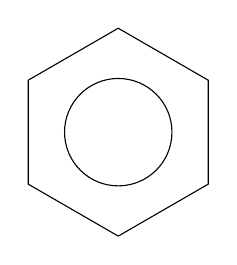
\begin{tikzpicture}[scale=1.1]
\draw (30:1.2) -- (90:1.2) -- (150:1.2) -- (210:1.2) -- (270:1.2) -- (330:1.2) -- cycle;
\draw (0,0) circle (0.62);
\end{tikzpicture}
\end{center}

上图是化学家常用的表示法：六边形代表 6 个碳组成的骨架，中间的圆圈代表那 6 个离域电子。这只是人为的记号——真实的分子没有线条也没有圆圈，只有一团以不同概率分布的电子云。

电子"跑圈"带来一个可以直接测量的后果：6 条碳碳键完全一模一样。普通碳碳单键长约 \ud{154}{pm}，双键约 \ud{134}{pm}；如果苯环里真的是单双键交替，键长就该一长一短交替。实测结果却是：6 条键全是 \ud{139}{pm}，整齐地介于单键和双键之间。6 个碳平起平坐，没有哪条键"更单"或"更双"。

\section{共振：画不下，只好画两张}

可问题来了。我们在纸面上画结构式，用的是第 17 章的规矩：一条线代表一对成键电子。苯环有 6 个离域电子，相当于 3 对双键电子，可它们不固定在任何两个碳之间——纸面上根本没有"画半条双键"这种操作。怎么办呢？化学家的办法是：画两张图。一张把双键画在 1、2 号碳之间，另一张把双键挪到 2、3 号碳之间，中间用一个双向箭头连起来，然后说：真实情况大约在这两张图"之间"。这两张图叫\textbf{共振式}，箭头叫共振箭头。

这里就是全章最容易掉进去的坑，也是本章的红线，请你把下面这句话读两遍：\textbf{苯分子并不是一半时间长成第一张图、另一半时间长成第二张图，更没有在两图之间来回翻转。}苯分子从诞生到消亡，每时每刻都是同一个样子——6 个电子均匀铺满整个环。那两张图里的任何一张，都从未真实存在过。

打个比方。你见过骡子，它是马和驴的后代。我可以这样向你描述骡子："它有点像马，又有点像驴。"但没有任何一头骡子会"一半时间是马、一半时间是驴"，更不会在马和驴之间来回切换——骡子每一秒都是骡子。马和驴只是你描述它时借用的两个参照物。两张共振式也是同样的道理：它们是记账工具，是我们有限的纸面符号对一种画不出来的真实结构的逼近。想明白这一点，你就比很多只会照抄"苯环在共振"这句话的人更懂苯。

那么，为什么偏偏要画两张，一张不够吗？不够。只画一张交替双键的图，就等于断言 6 条键有长有短、电子有固定位置——这与实测键长、与苯的稳定性全都对不上。两张（以及更多次要贡献的图）合起来，才勉强表达出"电子均匀摊开"这件事。符号迁就现实，而不是现实迁就符号。

\begin{qiaoliang}
电子离域到底给苯省了多少能量？做个"假想的对比实验"就知道了。环己烯只有一个双键，让它加氢变成环己烷，每个双键放热约 \ud{120}{kJ/mol}。如果苯环真是三个互不相干的普通双键，苯加氢就该放热 $3\times 120=360$ \ud{}{kJ/mol}。实际测量呢？只有约 \ud{208}{kJ/mol}。差值大约 \ud{150}{kJ/mol}——苯比"假想的三个双键"足足低了这么多能量。这部分多出来的稳定，就叫\textbf{离域能}（也常叫芳香稳定化能），它是 6 个电子跑圈"省下"的能量。用第 27 章的语言说：能量越低，体系越"懒得"变化。苯不肯像烯烃那样爽快加成，原因就在这里——加成会拆掉电子甜甜圈，得先赔上这 \ud{150}{kJ/mol}，得不偿失。
\end{qiaoliang}

\section{芳香性：稳定不是白来的}

化学家把苯环这种"环状、平面、电子绕环离域、因此格外稳定"的性质称为\textbf{芳香性}。注意，"稳定"永远是相对的（第 29 章的提醒）：苯不是不反应，而是挑食。它最喜欢的吃法是\textbf{取代}——环上一个氢被别的原子或基团顶掉，电子甜甜圈原封不动；而不是烯烃那种加成——加成要拆甜甜圈。于是苯的化学性格和烯烃几乎是反的：烯烃见到电子贫乏的试剂就扑上去加成，苯则慢悠悠地、在催化剂帮助下才肯发生取代。

芳香性不是苯的专利。后面你会看到，生命分子里到处是这样的环：DNA 里的碱基、蛋白质里的几种氨基酸侧链、你眼睛里感光的分子的关键部位，都含有芳香环或类似的离域体系。几亿年的演化反复选中这种结构，原因和化学家选中它的原因一样——稳定、平坦、尺寸合适，是搭分子机器的上好零件。

\section{给圆环挂上旋钮：取代基改变电子分布}

苯环像一个圆形的工作台，而工作台的脾气，取决于往上面挂什么。这些挂在环上的原子团叫\textbf{取代基}，它们做两件事：改变环上电子云的疏密分布，也给分子装上新的"反应接口"（第 37 章的官能团概念在这里直接续上）。

有的取代基像"推手"，把电子往环里送。比如羟基（\chem{-OH}）、氨基（\chem{-NH_2}）：它们让环上的电子云更密集，环变得更"电子富有"，也更容易吸引电子贫乏的试剂。有的取代基像"拉钩"，把电子从环里往外抽。比如硝基（\chem{-NO_2}）、羧基（\chem{-COOH}）：环被抽得电子稀疏，脾气随之改变。

别小看这点电子的推拉，它直接改写分子的性质。对比两个人都见过的物质：乙醇（第 40 章）和苯酚。两者都带羟基，可乙醇的水溶液是中性的，苯酚的水溶液却明显显弱酸性——因为羟基挂在苯环上时，氢离子脱落后剩下的负电荷可以摊进芳香环的离域体系里，被"大家"一起分担，所以氢更容易放手。同一个羟基，挂在链上是醇，挂在芳香环上就成了弱酸。结构决定电子分布，电子分布决定性格——这条因果链在第 32 章讲酸碱时埋过线，现在它在有机分子里再次显灵。

取代基还能决定一个新来的基团落在环的哪个位置：推手型取代基倾向于把它引到自己的邻位和对位，拉钩型的偏好则相反。合成药物和染料时，化学家就是靠这套"定位规则"规划反应顺序的——先挂谁、后挂谁，顺序错了就得到一堆位置不对的杂质。这背后没有口诀要背，只有一条逻辑：电子从哪里富足、哪里贫乏，反应就往哪里走。

\section{证据：六边形是怎样被拍下来的}

\begin{zhengju}
苯的六边形环结构，是 1865 年由凯库勒提出的。传说他从"蛇咬住自己尾巴"的梦境获得灵感——故事真假难辨，但可以确定的是，他生前始终没能解决那个矛盾：如果环里单双键交替，苯为什么不像烯烃那样爱加成？此后几十年，化学家提出过各种竞争结构：有人画棱柱形，有人画中心对角相连的结构，谁也说服不了谁。争论的裁判最终是两批互不相干的证据。

第一批来自晶体。1929 年，英国晶体学家凯瑟琳·朗斯代尔用 X 射线照射六甲基苯的晶体。X 射线遇到规则排列的原子会发生衍射，从衍射斑点的位置可以反推出原子在空间的排布（这套方法的思路，第 24 章介绍过）。结果清清楚楚：6 个碳排成平坦的正六边形，所有碳碳键等长。棱柱形之类的候选结构就此出局。

第二批来自热量，就是你前面算过的那笔账：苯加氢的放热比"三个普通双键"少了约 \ud{150}{kJ/mol}。如果苯只是两种结构飞快地来回切换，这种"切换"本身并不能解释能量为何凭空变低——分子又不是靠切换姿势省钱的。只有一种解释同时满足两批证据：电子本来就摊在整个环上，摊得越开，能量越低。后来量子力学的计算（第 9 章那套工具的延伸）精确复现了键长和能量，故事才算闭环。

请注意这个证据链的形状：先有一个好用但带硬伤的结构假说，再有互不相干的两类测量把候选者逐一排除，最后理论解释追上来补上"为什么"。它不是某个天才灵光一闪的瞬间，而是半个多世纪的拉锯。
\end{zhengju}
\section{染料为什么有颜色}

回到开场那条牛仔裤。白色药片和蓝色布料的分野，藏在电子能级的缝隙大小里。

回忆第 9 章：电子住在能量不同的"楼层"上，吸收恰好等于楼层差能量的光，电子就能跳上一级。苯环上的离域电子也有自己的楼层，但苯的楼层差比较大，对应的吸收落在紫外线区——人眼看不见紫外线，所以苯是无色的。要让分子显出颜色，就得把楼层差压缩到可见光的范围。

办法朴素得可爱：\textbf{把离域的"跑道"加长}。离域电子摊开的范围越大，楼层之间挤得越密，楼层差就越小，吸收的光就从紫外线一路挪进可见光区。一个苯环不够，就把两个环连起来，再插进一根同样能离域的"桥"——比如偶氮基（\chem{-N=N-}）。这类分子叫偶氮染料，占今天合成染料的大半壁江山。分子吸收掉可见光里的一段颜色，剩下的光混合起来进入你的眼睛，你看到的就是被吸收那段的\textbf{补色}：吸收橙光显蓝，吸收蓝光显黄。牛仔裤的靛蓝，正是一个吸收橙红光的长共轭分子。

取代基在这里再次当旋钮：给共轭链挂上羟基、氨基这类推手基团，楼层差还会被进一步微调，颜色随之深浅变化、红移蓝移。染整工程师调色，调的其实是分子结构。

做个数量级的直觉估算。可见光光子的能量大约在 $170$ 到 $300$ \ud{}{kJ/mol} 之间（把单个光子的能量乘上阿伏伽德罗常数），而苯的离域电子跃迁需要的能量比这更高，落在紫外区；共轭链每加长一段，能级差就缩一截，缩进 $170$–$300$ 这个窗口，颜色就出现了。你眼里整个色彩世界，本质上是一张"分子能级差分布图"。

这个原理是 1856 年被一个 18 岁的年轻人误打误撞揭开的。珀金本想用煤焦油里的原料合成抗疟疾药奎宁，反应失败，烧瓶里只剩一团黑泥。换个人可能就倒掉了，他却注意到黑泥能溶出漂亮的紫色，还能把布料染得结实鲜亮——世界上第一种合成染料"苯胺紫"就此诞生。短短几十年，围绕煤焦油和芳香环长出了一个庞大的合成染料工业，人类第一次不必靠捣碎的植物和虫子给布料上色。顺便说，奎宁后来也被合成了，但那是更晚、更曲折的故事。

颜色也不是永恒的。染料分子的共轭链怕强光和氧：阳光中的紫外线加上空气中的氧，会一点点咬断共轭链，楼层差重新变大，布料就褪色了。这就是为什么阳台边的窗帘朝外一面总是先变白。

\section{药物：一个芳香环的身体之旅}

现在轮到药片。以对乙酰氨基酚为例，它的分子里有一个苯环，环的对位挂着一个羟基和一个酰胺基。这颗药进嘴之后要走四关，每一关的成败都写在分子结构上。

第一关是\textbf{溶解}。药得先溶进胃肠道的液体——主要是水——才能被吸收。芳香环是"油性"的：碳氢骨架跟水合不来（第 22、23 章讲的分子间作用力），所以纯芳香化合物大多难溶于水。羟基和酰胺基是极性基团，能和水分子拉氢键，是分子自带的"亲水把手"。一颗好药往往是油性与水性的精确配比：太亲水，穿不过下一关的细胞膜；太亲油，连水都溶不进去。

第二关是\textbf{吸收与运输}。细胞膜是一层油性的屏障（第 51 章会细讲它的结构），分子得有点"油性"才混得过去。苯环这截碳氢骨架恰好提供了这部分通行证。

第三关是\textbf{结合}。药要起效，通常得嵌进某个蛋白质表面的凹陷，形状互补、电荷相合，像钥匙进锁——详细机制属于第 48、49 章。芳香环在这里的贡献是：平坦、刚性、尺寸固定的骨架。柔性链条分子会扭来扭去，吻合只是碰运气；刚性芳香环则像一把形状确定的钥匙坯子，碰上对的锁就能稳稳卡住。环上取代基的位置，决定了"钥匙齿"的形状。

第四关是\textbf{代谢}。身体把外来分子当作需要处理的对象，肝脏里的酶（本质是蛋白质催化剂，第 30 章和第 49 章的规则全部适用）会给芳香环"打孔"——把羟基等极性基团装上去，把油性分子改造成水溶性更好的分子，最后经肾脏随尿排出。代谢快慢直接决定药效持续多久，也决定\textbf{剂量}。对乙酰氨基酚在常规剂量下，绝大部分被安全地代谢掉；但剂量过大时，一条次要的代谢路径会被迫开足马力，产生一种会耗竭肝脏防护物质的有毒中间产物——这就是"常用药过量也会出大事"的分子层面的原因。同一分子，剂量不同，结局不同；而且每个人的酶活性、体重、肝脏状况都不一样，所以剂量这件事永远属于医生和说明书，不属于"我觉得"。本章谈药只谈原理，具体用药请遵医嘱。

你看，溶解、吸收、结合、代谢、剂量——一颗药丸的设计，全是在分子结构上做加减法：这里加个环稳形状，那里挂个羟基调溶解，再留一个代谢的"出口"。这套思路属于第 44 章的有机合成世界，那里会讲化学家怎样倒推着把这样的分子搭出来。

\section{这套模型哪里会失灵}

诚实的时间到了。本章给了你三样工具：离域电子的图景、共振式符号、"结构决定性质"的逻辑。它们各有边界。

离域图景说的是"电子摊得越开越稳定"，但"摊开"需要几何条件：环得足够平，轨道才能肩并肩叠上。有些环状分子明明画得出交替单双键，却因为扭成非平面形状而享受不到这份稳定——电子云叠不上，芳香性就是空谈。

共振式是记账工具，不是分子照片。它能帮你数电子、估分布，但谁要是拿着两张共振式追问"此刻分子是哪一张"，那就是把地图当成了领土——本章红线在此。

最需要克制的是"结构决定性质"外推到药效。结构能告诉你溶解性的大致方向、提供结合的候选形状、提示可能的代谢位点，但生物体是一整座化学城市（第 45 章起你会看到全貌），同样的骨架接在不同的分子上、进入不同的身体，效果可能南辕北辙。结构给出的是倾向，不是判决书。这就是为什么新药必须经过一层又一层的实验验证，而不能靠图纸封神。

\begin{wuqu}
"苯分子在两种结构之间快速来回切换，所以平均下来键长一样。"——这是流传极广的误解，甚至连"互变异构"的实验现象都会让人产生类似联想。反例有两个。其一，切换解释不了能量：两种结构来回跳，体系能量不会因此降低 \ud{150}{kJ/mol}，可实测的加氢热明明白白少了这么多——只有"电子本来就摊开"才能解释这笔省下来的能量。其二，切换预言了烯烃脾气：哪怕只在一瞬间以"含双键"的形态存在，苯也该像烯烃一样让溴水褪色，可它偏不。苯分子每一刻都是那副"四不像"的完整样子；切换的是我们纸上的画法，不是分子本身。
\end{wuqu}

\begin{shiyan}
\textbf{观察"油性和水性"：色素站队实验}（在家可做）

材料：两个透明玻璃杯、清水、少量食用油、食用色素一小瓶（或一滴红蓝墨水）、一根筷子。

步骤：① 两只杯子各装半杯水，各滴入 1 滴色素，搅匀，记下颜色深浅。② 向其中一杯缓缓倒入约两勺食用油，静置片刻观察分层。③ 用筷子轻轻搅动后静置，观察色素分子去了哪一层。④ 另取白纸，把两杯液体分别蘸一点滴在纸上，对比颜色。

观察点：色素分子大多带极性基团（否则没法溶于水），你会看到颜色几乎全部留在水层，油层基本不染——这就是"极性拉手"决定溶解去向的直观版本，也正是药物设计里"亲水还是亲油"的第一道选择题。

安全提示：食用色素安全但极难洗，垫好报纸，别穿浅色衣服操作；实验液体不可饮用，结束后洗手。
\end{shiyan}

\section{回到药片和牛仔裤}

现在兑现开场的承诺。那颗白色药片：苯环给了分子一块平坦刚性的骨架，好让它有确定的形状去配蛋白质的锁孔；环上的羟基和酰胺基是亲水把手和代谢出口，决定它溶得多快、起效多久、以什么剂量才安全。白是因为它只吸收紫外线——共轭太短，够不着可见光。

那条蓝牛仔裤：靛蓝分子把离域跑道修得足够长，能级差缩进可见光窗口，橙红光被吸收，蓝光被留下。它是 19 世纪从煤焦油出发的染料工业的直系后代，也会被阳光和氧慢慢咬断跑道而褪色。

一个六边形环，两种完全不同的用法：药用的是它的\textbf{形状}，染料用的是它的\textbf{电子能级}。同一种结构原则，撑起两个庞大的产业——这就是"组成部分怎样连接和排列"这条追问（贯穿问题之二）的威力。

\section{平面之外，还有左右手}

本章的芳香环是平的。但你身体里几乎每一个重要分子——糖、氨基酸、药物靶点——都是立体的，而且很多立体结构存在一种微妙的对称：像左手和右手，互为镜像却永远无法重合。两"只手"的分子，组成完全一样、连接顺序完全一样，唯独空间朝向相反；而在生命这台精密机器里，左手和右手的待遇可以天差地别：一个治病，另一个可能无效，甚至有害。下一章，我们就来认识这对最微妙的双胞胎。

\begin{tiaozhan}
什么样的环才有资格"芳香"？1931 年休克尔给出一个数电子的规则：平面环状的离域体系，当参与跑圈的电子数等于 $4n+2$（$n$ 取 0、1、2……）时格外稳定。苯有 6 个离域电子，$6=4\times 1+2$，芳香；环丁二烯只有 4 个电子，$4=4\times 1$，不在"优惠名单"上，它极度不稳定，化学家要用极低温才能把它留住观察；萘（卫生球的旧配方成分）两个环共用 10 个电子，$10=4\times 2+2$，同样芳香。为什么会有这样古怪的数字？答案藏在量子力学里：环上离域电子的能级排布像一圈座位，$4n+2$ 恰好对应"座位成对坐满、没有半满的尴尬"的闭壳层局面——和第 9 章原子里"住满的楼层格外安稳"是同一套逻辑在分子尺度的重演。这部分跳过不影响主线，但如果你曾好奇"6 有什么特别"，现在你知道了。
\end{tiaozhan}

\section*{练一练}

\begin{sikaoti}
\item 画两个图：先画苯环的"两张共振式"（双键位置交替的两张结构），再画化学家常用的"六边形加圆圈"表示法。在每个图旁各写一句话：这张图能表达什么、表达不了什么？
\item 环己烯加一个氢分子放热约 \ud{120}{kJ/mol}。若某假想分子"环己三烯"有三个互不相干的双键，预期加氢放热多少？实测苯只有约 \ud{208}{kJ/mol}。用能量语言解释这个差值，并据此预言：苯和环己烯，谁更容易发生加成反应？
\item 苯酚（羟基挂在苯环上）显弱酸性，乙醇（羟基挂在碳链上）接近中性。用"负电荷能否摊进离域体系"这个思路，画一张示意图解释两者的差别。
\item 某种黄色染料吸收蓝光。工程师在它的共轭链上再接一个苯环，把离域跑道加长。预言：它的吸收峰会移向更长的波长还是更短的波长？颜色可能向哪个方向变化？
\item 某药物分子油性强、几乎不溶于水，口服吸收很差。药剂师在它的分子上引入一个带负电的极性基团制成盐。从"溶解—过膜"两关的角度，分析这个改动会带来什么好处、又可能付出什么代价。
\item 一位同学说："苯的两种共振结构各占一半时间，所以测出的键长是平均值。"请用本章的两个实验事实反驳他，并给出正确的表述。
\end{sikaoti}
